% !TeX program = xelatex
\documentclass[10pt]{beamer}

\usetheme{metropolis}

\usepackage{pgfplots}
\usepgfplotslibrary{fillbetween}
\usepackage{pgfopts}
\usepackage{amsmath}
\usepackage{structuralanalysis}
\usepackage{tikz}
\usepackage{tikz-3dplot}
\usepackage{chngcntr}
\usepackage{wasysym}
\usepackage{mathtools}
\usepackage{alphalph}
\usepackage{xcolor}
\usepackage[showdow=false, en-US]{datetime2}

\newcommand{\highlight}[1]{%
	\colorbox{red!50}{$\displaystyle#1$}}

\setcounter{lecture}{8}
\counterwithin{equation}{lecture}
\makeatletter
\def\user@resume{resume}
\def\user@intermezzo{intermezzo}
%
\newcounter{previousequation}
\newcounter{lastsubequation}
\newcounter{savedparentequation}
\setcounter{savedparentequation}{1}
% 
\renewenvironment{subequations}[1][]{%
	\def\user@decides{#1}%
	\setcounter{previousequation}{\value{equation}}%
	\ifx\user@decides\user@resume 
	\setcounter{equation}{\value{savedparentequation}}%
	\else  
	\ifx\user@decides\user@intermezzo
	\refstepcounter{equation}%
	\else
	\setcounter{lastsubequation}{0}%
	\refstepcounter{equation}%
	\fi\fi
	\protected@edef\theHparentequation{%
		\@ifundefined {theHequation}\theequation \theHequation}%
	\protected@edef\theparentequation{\theequation}%
	\setcounter{parentequation}{\value{equation}}%
	\ifx\user@decides\user@resume 
	\setcounter{equation}{\value{lastsubequation}}%
	\else
	\setcounter{equation}{0}%
	\fi
	\def\theequation  {\theparentequation  \alph{equation}}%
	\def\theHequation {\theHparentequation \alph{equation}}%
	\ignorespaces
}{%
%  \arabic{equation};\arabic{savedparentequation};\arabic{lastsubequation}
\ifx\user@decides\user@resume
\setcounter{lastsubequation}{\value{equation}}%
\setcounter{equation}{\value{previousequation}}%
\else
\ifx\user@decides\user@intermezzo
\setcounter{equation}{\value{parentequation}}%
\else
\setcounter{lastsubequation}{\value{equation}}%
\setcounter{savedparentequation}{\value{parentequation}}%
\setcounter{equation}{\value{parentequation}}%
\fi\fi
%  \arabic{equation};\arabic{savedparentequation};\arabic{lastsubequation}
\ignorespacesafterend
}
\makeatother
\title{AE 737 - Mechanics of Damage Tolerance}
\subtitle{Lecture \arabic{lecture}}
\date{Last Updated: \today\ at \DTMcurrenttime}
\author{Dr. Nicholas Smith}
\institute{Wichita State University, Department of Aerospace Engineering}
% \titlegraphic{\hfill\includegraphics[height=1.5cm]{logo/logo}}

\begin{document}

\maketitle

\begin{frame}{homework review}
	\begin{itemize}
		\item $K_{Ie} > K_I$
		\item Sanity check on plots
		\item Significant figures
		\item polar plots in Excel - convert to x,y, set axis scales to be equivalent
		\item watch out for "smoothing" in Excel (add more data points)
	\end{itemize}
\end{frame}

\begin{frame}{schedule}
	\begin{itemize}
		\item 16 Feb - Residual Strength, Homework 3 Due, Homework 4 Assigned
		\item 18 Feb - Residual Strength
		\item 23 Feb - Multiple Site Damage, Homework 4 Due, Homework 5 Assigned
		\item 25 Feb - Mixed-mode Fracture
		\item 1 Mar - Section 1 Review, Homework 5 Due
		\item 3 Mar - Section 1 Review, Homework 5 return
		\item 8 Mar - Exam 1
		\item 10 Mar - Exam return, Final Project discussion
	\end{itemize}
\end{frame}

\begin{frame}
  \frametitle{outline}
  \setbeamertemplate{section in toc}[sections numbered]
  \tableofcontents[hideallsubsections]
\end{frame}

\section{compounding}
\begin{frame}{compounding}
	\begin{itemize}
		\item Different types of boundaries create different correction factors to the usual stress intensity factor
		\item We often use $\beta$ to indicate the total correction factor
		\item When multiple boundaries are present, we can combine them into one effective correction factor
		\item There are two general methods we use to create a compound correction factor
	\end{itemize}
\end{frame}

\begin{frame}{compounding method 1}
	\begin{itemize}
		\item The first method uses linear superposition, and thus is restricted to cases where the effect of each boundary can be assumed to add linearly
		\item While in most cases this is not strictly true, it provides a reasonable approximation
		\begin{equation}
		K_r = \bar{K} + \sum_{i=1}^{N}(K_i - \bar{K})
		\end{equation}
		\item Where $N$ is the number of boundaries, $\bar{K}$ is the stress intensity factor with no boundaries present and $K_i$ is the stress intensity factor associated with the $i^{\text{th}}$ boundary.
	\end{itemize}
\end{frame}

\begin{frame}{compounding method 1}
	\begin{itemize}
		\item We can rewrite this equation as
		\begin{equation}
		K_r = \sigma \sqrt{\pi a} \beta_r = \sigma \sqrt{\pi a} + \sum_{i=1}^{N}(\sigma \sqrt{\pi a}\beta_i - \sigma \sqrt{\pi a})
		\end{equation}
		\item Which leads to an expression for $\beta_r$ as
		\begin{equation}
		\beta_r = 1+\sum_{i=1}^{N} (\beta_i - 1)
		\end{equation}
	\end{itemize}
\end{frame}

\begin{frame}{compounding method 2}
	\begin{itemize}
		\item An alternative empirical method approximates the boundary effect as
		\begin{equation}
		\beta_r = \beta_1 \beta_2 ... \beta_N
		\end{equation}
		\item If there is no interaction between the boundaries, method 1 and method 2 will give the same result
	\end{itemize}
\end{frame}
%Hand-draw examples from book

\begin{frame}{group 1}
		\begin{figure}[H]
			\centering
			\begin{tikzpicture}
			\begin{scope}[scale=1.5]
			\point{a}{0}{2};
			\point{b}{3}{2};
			\point{c}{0}{-3};
			\point{d}{3}{-3};
			\draw (0,0) -- (0,1) -- (2,1) -- (2,-1) -- (0,-1) -- (0,0);
			\draw (0.2,0) -- (0.8,0);
			\draw node at (0.15,0.1) {\small A} node at (.85,.1) {\small B} node at (.25,.5) {\small $b$};
			\draw node at (0.5,-0.2) {2a};
			\lineload{3}{a}{b}[-.5][-.5];
			\draw node at (1,2) {$\sigma$};
			\lineload{3}{c}{d}[.5][.5];
			\draw node at (1,-2) {$\sigma$};
			\draw[->] (0.7,-0.7) -- (0,-0.7);
			\draw[->] (1.3,-0.7) -- (2,-0.7);
			\draw node at (1,-0.7) {$W$};
			\draw[dashed] (.5,0) -- (.5,.8);
			\draw[->] (0.15,.5) -- (0,.5);
			\draw[->] (.35,.5) -- (.5,.5);
			\draw node at (2.2,0) {$2h$};
			\draw[->] (2.2,0.5) -- (2.2,1);
			\draw[->] (2.2,-0.5) -- (2.2,-1);
			\end{scope}
			\end{tikzpicture}
			\caption{off-center crack, finite height, $2h=1.6$, $b=.75$, $2a=1.2$, $W=4$}
		\end{figure}
\end{frame}
%off-center crack, finite height

\begin{frame}{group 2}
	\begin{figure}[H]
		\centering
		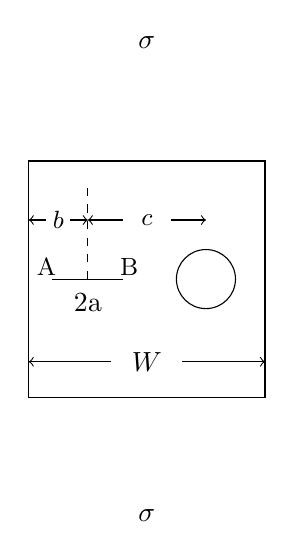
\begin{tikzpicture}
		\begin{scope}[scale=1.5]
		\point{a}{0}{2};
		\point{b}{3}{2};
		\point{c}{0}{-3};
		\point{d}{3}{-3};
		\draw (0,0) -- (0,1) -- (2,1) -- (2,-1) -- (0,-1) -- (0,0);
		\draw (0.2,0) -- (0.8,0);
		\draw node at (0.15,0.1) {\small A} node at (.85,.1) {\small B} node at (.25,.5) {\small $b$} node at (1,0.5) {\small $c$};
		\draw node at (0.5,-0.2) {2a};
		\lineload{3}{a}{b}[-.5][-.5];
		\draw node at (1,2) {$\sigma$};
		\lineload{3}{c}{d}[.5][.5];
		\draw node at (1,-2) {$\sigma$};
		\draw[->] (0.7,-0.7) -- (0,-0.7);
		\draw[->] (1.3,-0.7) -- (2,-0.7);
		\draw node at (1,-0.7) {$W$};
		\draw[dashed] (.5,0) -- (.5,.8);
		\draw[->] (0.15,.5) -- (0,.5);
		\draw[->] (.35,.5) -- (.5,.5);
		\draw[<-] (0.5,.5) -- (0.8,.5);
		\draw[->] (1.2,.5) -- (1.5,.5);
		\draw (1.5,0) circle (0.25);
		\end{scope}
		\end{tikzpicture}
		\caption{off-center crack, near a hole, $b=0.5$, $2a=0.6$, $R=1.17$, $c=1.67$, $W=4$}
	\end{figure}
\end{frame}
%off-center crack, near hole

\begin{frame}{group 3}
	\begin{figure}[H]
		\centering
		\begin{tikzpicture}
		\begin{scope}[scale=1.5]
		\point{a}{0}{2};
		\point{b}{6}{2};
		\point{c}{0}{-3};
		\point{d}{6}{-3};
		\draw (0,0) -- (0,1) -- (4,1) -- (4,-1) -- (0,-1) -- (0,0);
		\draw (1.5,0) -- (2.5,0);
		\draw node at (2,0.2) {2a};
		\lineload{3}{a}{b}[-.5][-.5];
		\draw node at (2,2) {$\sigma$};
		\lineload{3}{c}{d}[.5][.5];
		\draw node at (2,-2) {$\sigma$};
		\draw (3,0) circle (0.25);
		\draw node at (1,0) {$2h$};
		\draw[->] (1,0.5) -- (1,1);
		\draw[->] (1,-0.5) -- (1,-1);
		\draw[->] (2.3,0.5) -- (2,0.5);
		\draw[->] (2.7,0.5) -- (3,0.5);
		\draw node at (2.5,0.5) {\small $c$};
		\end{scope}
		\end{tikzpicture}
		\caption{centered crack, near a hole, finite height, $2a=2$, $W=4$, $2h=2$, $R=0.25$, $c=1.5$}
	\end{figure}
\end{frame}
%centered crack, near hole, finite height

\begin{frame}{group 4}
	\begin{figure}[H]
		\centering
		\begin{tikzpicture}
		\begin{scope}[scale=1.5]
		\point{a}{0}{2};
		\point{b}{6}{2};
		\point{c}{0}{-3};
		\point{d}{6}{-3};
		\draw (0,0) -- (0,1) -- (4,1) -- (4,-1) -- (0,-1) -- (0,0);
		\draw (1.5,0) -- (2.5,0);
		\draw node at (2,0.2) {2a};
		\lineload{3}{a}{b}[-.5][-.5];
		\draw node at (2,2) {$\sigma$};
		\lineload{3}{c}{d}[.5][.5];
		\draw node at (2,-2) {$\sigma$};
		\draw (3,0) circle (0.25);
		\draw (1,0) circle (0.35);
		\draw[->] (2.3,0.5) -- (2,0.5);
		\draw[->] (2.7,0.5) -- (3,0.5);
		\draw node at (2.5,0.5) {\small $c_2$};
		\draw[->] (1.3,0.5) -- (1,0.5);
		\draw[->] (1.7,0.5) -- (2,0.5);
		\draw node at (1.5,0.5) {\small $c_1$};
		\end{scope}
		\end{tikzpicture}
		\caption{centered crack, near two holes, $2a=2$, $R_1=0.5$, $c_1=1.75$, $R_2=0.375$, $c_2=1.875$}
	\end{figure}
\end{frame}
%centered crack, near two holes

\section{thickness effects}

\begin{frame}{thickness effects}
	\begin{itemize}[<+->]
		\item We already know there is a difference between plane strain and plane stress fracture toughness
		\item As a material gets thicker and thicker, it converges to the plane strain solution
		\item Thinner specimens tend towards the plane stress solution
		\item When a specimen is thinner than some critical thickness, the material behavior is somewhat unknown
		\item Some materials retain the constant plane stress fracture toughness
		\item Others exhibit an unpredictable decrease in fracture toughness
		\item The phenomenon is not well-understood
	\end{itemize}
\end{frame}

\begin{frame}{thickness effects}
	\begin{itemize}[<+->]
		\item There is also a difference in the fracture surface between thin and thick specimens
		\item Thin specimens (in plane stress region) fail due to slant fracture
		\item This actually indicates some mixed-mode conditions at failure
		\item Thick specimens fail due to square fracture (with a small shear tip near the edges)
		\item This is more consistent with pure Mode I
	\end{itemize}
\end{frame}

\begin{frame}{slant fracture}
\begin{figure}
\centering
\includegraphics[width=0.7\linewidth]{slant}
\label{fig:slant}
\end{figure}
\end{frame}

\begin{frame}{shear lip}
\begin{figure}
\centering
\includegraphics[width=0.7\linewidth]{shear_lip}
\label{fig:shear_lip}
\end{figure}
\end{frame}

\section{residual strength}

\begin{frame}{residual strength}
	\begin{itemize}[<+->]
		\item In the last chapter we performed some basic residual strength analysis by checking for net section yield
		\item As the crack grows, the area of the sample decreases, increasing the net section stress
		\item The residual strength, $\sigma_R$ is given in terms of the gross area, so as the crack grows the residual strength due to yield decreases
		\item We can relate the net-section stress to $\sigma_R$ by
		\begin{equation}
		\sigma_R = \sigma_{YS} \frac{A_{net}}{A_{gross}}
		\end{equation}
	\end{itemize}
\end{frame}

\begin{frame}{residual strength}
	\begin{figure}
		\begin{tikzpicture}
		\begin{axis}[domain=0:1,
		xlabel=$a/W$,
		ylabel=Residual Strength $\sigma_R$,
		ytick={0, 2},
		yticklabels={0, $\sigma_{YS}$ }]
		\addplot[mark=none,style=dashed] {-2*x + 2};
		\end{axis}
		\end{tikzpicture}
	\end{figure}
\end{frame}

\begin{frame}{residual strength}
	\begin{itemize}[<+->]
		\item For brittle fracture to occur, we need to satisfy the condition
		\item
		\begin{equation}
		\sigma_R = \sigma_C = \frac{K_C}{\sqrt{\pi a}\beta}
		\end{equation}
	\end{itemize}
\end{frame}

\begin{frame}{residual strength}
	\begin{figure}
		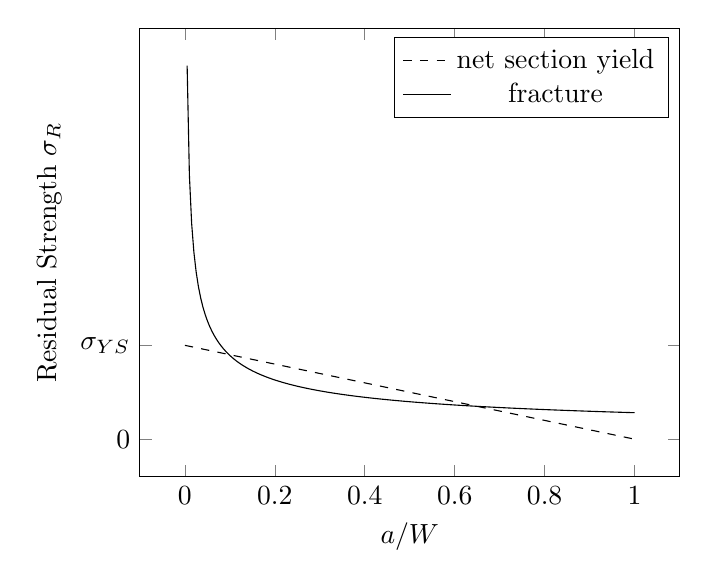
\begin{tikzpicture}
		\begin{axis}[domain=0:1,
		samples=200,
		xlabel=$a/W$,
		ylabel=Residual Strength $\sigma_R$,
		ytick={0, 2},
		yticklabels={0, $\sigma_{YS}$ }]
		\addplot[mark=none,style=dashed] {-2*x + 2};
		\addlegendentry{net section yield}
		\addplot[mark=none] {1/sqrt(3.14*x)};
		\addlegendentry{fracture}
		\end{axis}
		\end{tikzpicture}
	\end{figure}
\end{frame}

\begin{frame}{residual strength}
	\begin{itemize}[<+->]
		\item Within the same family of materials (i.e. Aluminum), there is generally a trade-off between yield stress and fracture toughness
		\item As we increase the yield strength, we decrease the fracture toughness (and vice versa)
		\item Consider a comparison of the following aluminum alloys
		\begin{enumerate}
			\item 7178-T6, $K_C = 43 \text{ ksi} \sqrt{\text{in.}}$, $\sigma_{YS} = 74 \text{ksi}$
			\item 7075-T6, $K_C = 68 \text{ ksi} \sqrt{\text{in.}}$, $\sigma_{YS} = 63 \text{ksi}$
			\item 2024-T3, $K_C = 144 \text{ ksi} \sqrt{\text{in.}}$, $\sigma_{YS} = 42 \text{ksi}$
		\end{enumerate}
	\end{itemize}
\end{frame}

\begin{frame}{residual strength}
	\begin{itemize}[<+->]
		\item As an example let us consider an edge-cracked panel with $W=6"$ and $t=0.1"$
		\item The net section yield condition will be given by
		\item 
		\begin{equation*}
		\sigma_C = \sigma_{YS} \frac{W-a}{W} = \sigma_{YS}\frac{6-a}{6}
		\end{equation*}
		\item And the fracture condition by
		\begin{equation*}
		\sigma_C = \frac{K_C}{\sqrt{\pi a} \beta}
		\end{equation*}
		With
		\begin{equation*}
		\beta = 1.12 - 0.231\left(\frac{a}{W}\right) + 10.55 \left(\frac{a}{W}\right)^2 - 21.72 \left(\frac{a}{W}\right)^3 + 30.39 \left(\frac{a}{W}\right)^4
		\end{equation*}
	\end{itemize}
\end{frame}

\begin{frame}{7178-T6}
	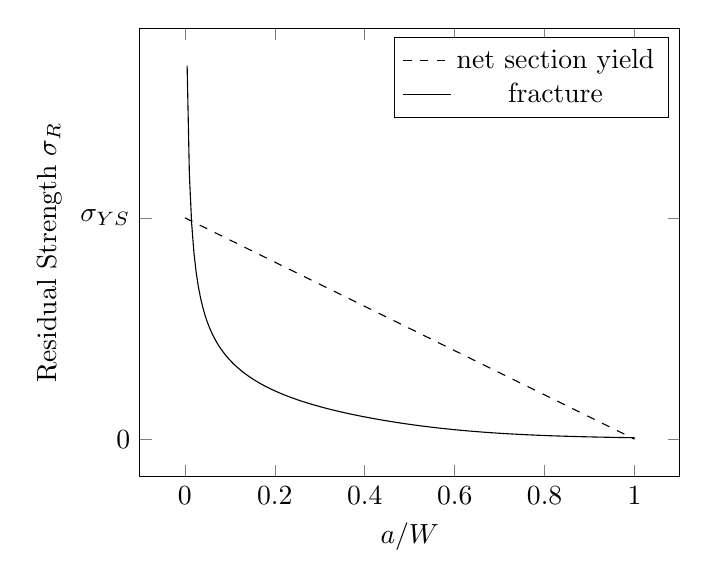
\begin{tikzpicture}
	\begin{axis}[domain=0:1,
	samples=200,
	xlabel=$a/W$,
	ylabel=Residual Strength $\sigma_R$,
	ytick={0, 74},
	yticklabels={0, $\sigma_{YS}$ }]
	\addplot[mark=none,style=dashed] {74*(1-x)};
	\addlegendentry{net section yield}
	\addplot[mark=none] {43/sqrt(3.14*x*6)/(1.12-.231*x+10.55*x^2-21.72*x^3+30.39*x^4)};
	\addlegendentry{fracture}
	\end{axis}
	\end{tikzpicture}
\end{frame}

\begin{frame}{7075-T6}
	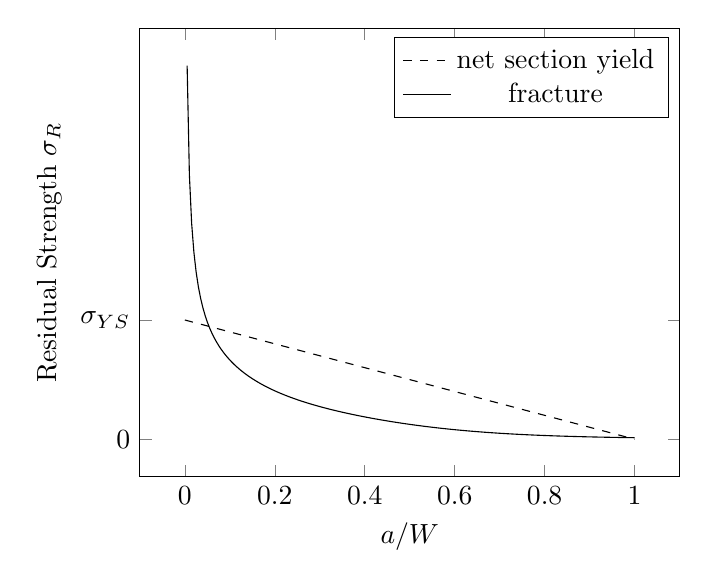
\begin{tikzpicture}
	\begin{axis}[domain=0:1,
	samples=200,
	xlabel=$a/W$,
	ylabel=Residual Strength $\sigma_R$,
	ytick={0, 63},
	yticklabels={0, $\sigma_{YS}$ }]
	\addplot[mark=none,style=dashed] {63*(1-x)};
	\addlegendentry{net section yield}
	\addplot[mark=none] {68/sqrt(3.14*x*6)/(1.12-.231*x+10.55*x^2-21.72*x^3+30.39*x^4)};
	\addlegendentry{fracture}
	\end{axis}
	\end{tikzpicture}
\end{frame}

\begin{frame}{2024-T3}
	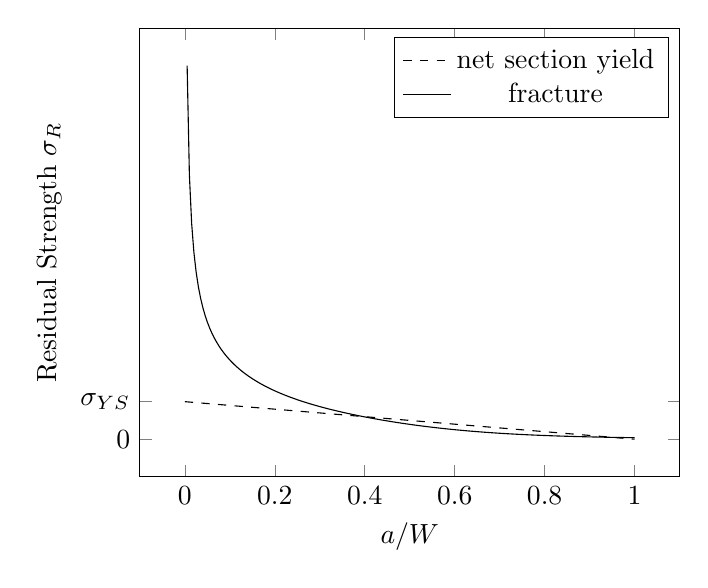
\begin{tikzpicture}
	\begin{axis}[domain=0:1,
	samples=200,
	xlabel=$a/W$,
	ylabel=Residual Strength $\sigma_R$,
	ytick={0, 42},
	yticklabels={0, $\sigma_{YS}$ }]
	\addplot[mark=none,style=dashed] {42*(1-x)};
	\addlegendentry{net section yield}
	\addplot[mark=none] {144/sqrt(3.14*x*6)/(1.12-.231*x+10.55*x^2-21.72*x^3+30.39*x^4)};
	\addlegendentry{fracture}
	\end{axis}
	\end{tikzpicture}
\end{frame}

\begin{frame}{comparison}
	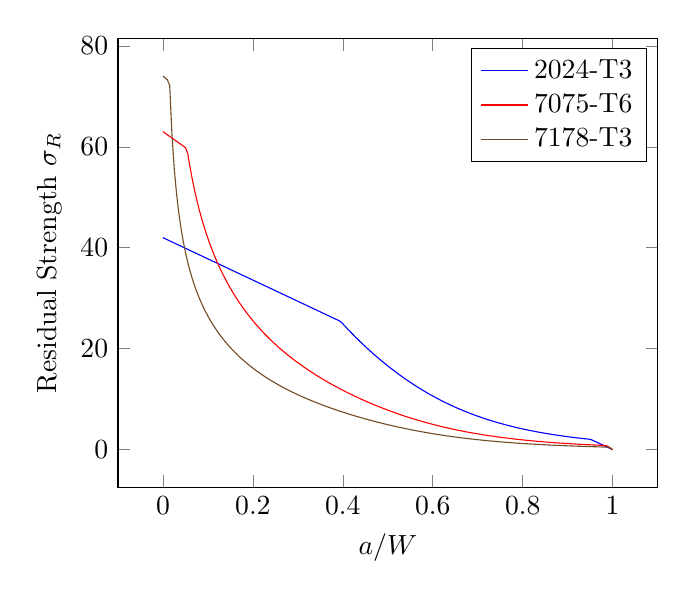
\begin{tikzpicture}
	\begin{axis}[domain=0:1,
	samples=200,
	xlabel=$a/W$,
	ylabel=Residual Strength $\sigma_R$]
	\addplot +[mark=none] {min(42*(1-x),144/sqrt(3.14*x*6)/(1.12-.231*x+10.55*x^2-21.72*x^3+30.39*x^4))};
	\addlegendentry{2024-T3}
	\addplot +[mark=none] {min(63*(1-x),68/sqrt(3.14*x*6)/(1.12-.231*x+10.55*x^2-21.72*x^3+30.39*x^4))};
	\addlegendentry{7075-T6}
	\addplot +[mark=none] {min(74*(1-x),43/sqrt(3.14*x*6)/(1.12-.231*x+10.55*x^2-21.72*x^3+30.39*x^4))};
	\addlegendentry{7178-T3}
	\end{axis}
	\end{tikzpicture}
\end{frame}

\begin{frame}{using MIL-handbook}
	\begin{itemize}[<+->]
		\item Uses a different grain nomenclature
		\item
		\begin{tabular}{c c}
			 $K_C$ & $\sigma_{YS}$ \\ 
			\hline 
			L-T  & L \\ 
			T-L  & L-T
		\end{tabular} 
		\item A-Basis vs. B-Basis values are reported (A = 99\% of population will meet/exceed value, B = 90\% of population)
		\item S-Basis - no statistical information available, standard value to be used
	\end{itemize}
\end{frame}

\begin{frame}{using MIL-handbook}
	\begin{itemize}
		\item $F_{tu}$ - ultimate tensile strength
		\item $F_{ty}$ - tensile yield strength
		\item $F_{cy}$ - compressive yield strength
		\item $F_{su}$ - ultimate shear strength
		\item $F_{bru}$ - ultimate bearing strength
		\item $F_{bry}$ - bearing yield strength
		\item $E$ - tensile Young's Modulus
		\item $E_c$ - compressive Young's Modulus
		\item $G$ - shear modulus
		\item $\mu$ - Poisson's ratio
	\end{itemize}
\end{frame}

\section{fedderson approach}

\begin{frame}{Fedderson approach}
	\begin{itemize}[<+->]
		\item Unfortunately, the method we described above does not quite match experimental results
		\item Fedderson proposed an alternative, where we connect the net-section yield and brittle fracture curves with a tangent line
		\item This approach agrees very well with experimental data
		\item Note: We could do something similar when the crack is very long, but we are generally less concerned with this region (failure will have already occurred)
	\end{itemize}
\end{frame}

\section{proof testing}

\begin{frame}{proof testing}
	\begin{itemize}[<+->]
		\item Proof testing is a way to use the concept of residual strength to check the size of a defect from manufacturing
		\item Due to the fatigue life of a certain panel, and/or an inspection cycle that we have prescribed for that part, we determine an "acceptable" initial flaw size, $a_0$
		\item We then determine a load which would cause failure at this crack length
		\item This is the "proof load"
		\item If the part does not fail in the proof test, we can assume that the largest flaw in the material is $a_0$
	\end{itemize}
\end{frame}

\begin{frame}{example}
	\begin{itemize}
		\item Suppose we are concerned about edge cracks in a panel with $\sigma_{YS} = 65 \text{ksi}$, $W=5"$
		\item We have determined that the largest allowable crack is 0.4"
		\item The fracture toughness of this panel is $K_c = 140 \text{ ksi} \sqrt{\text{in.}}$
		\item We can find the proof load
		\begin{align*}
		\sigma_c &= \frac{K_c}{\sqrt{\pi a_0} \beta}\\
		&= \frac{140}{\sqrt{\pi 0.4} (1.161)}\\
		&= 107.6
		\end{align*}
		\item So the proof load would need to induce a gross section stress of 107.6 ksi.
	\end{itemize}
\end{frame}
\end{document}
